\chapter{Results of the Measurements and Evaluation of the Simulation} \label{sec:cha6}
The buck converter of the previous chapter is now measured and its results are presented to show the efficiency behaviour of the inductor. The resulting measurements are assessed for expected behaviour and interpreted. Based on the comparison to the simulation results, the ability of the simulation to approximate the efficiency behaviour is validated.

\section{Results of the Buck Converter Measurements}\label{sec:results_of_the_bc_measurement}
Measuring the buck converter is done 20 times, once for each possible combination of inductor and \ac{GaNFET}. The input voltage is checked every measurement to ensure a constant \SI{30}{V} supply to the \ac{HS} \ac{GaNFET}. By doing so the comparison to the simulation can be made more easily, as it does not take into account a voltage drop occurring between the source and \ac{HS} \ac{GaNFET}, caused by the impedance of the \ac{PCB}.\\
The efficiency of the buck converter is given by
\begin{equation}
    \eta = \frac{\text{Power output to the load}}{\text{Power input by the power supply}} \quad\text{.}
\end{equation}
Comparing the efficiency for the different inductors while using the \textit{EPC2088} qualitatively shows the frequency-dependent behaviour of the losses. 
\begin{figure}[H]
    \centering
    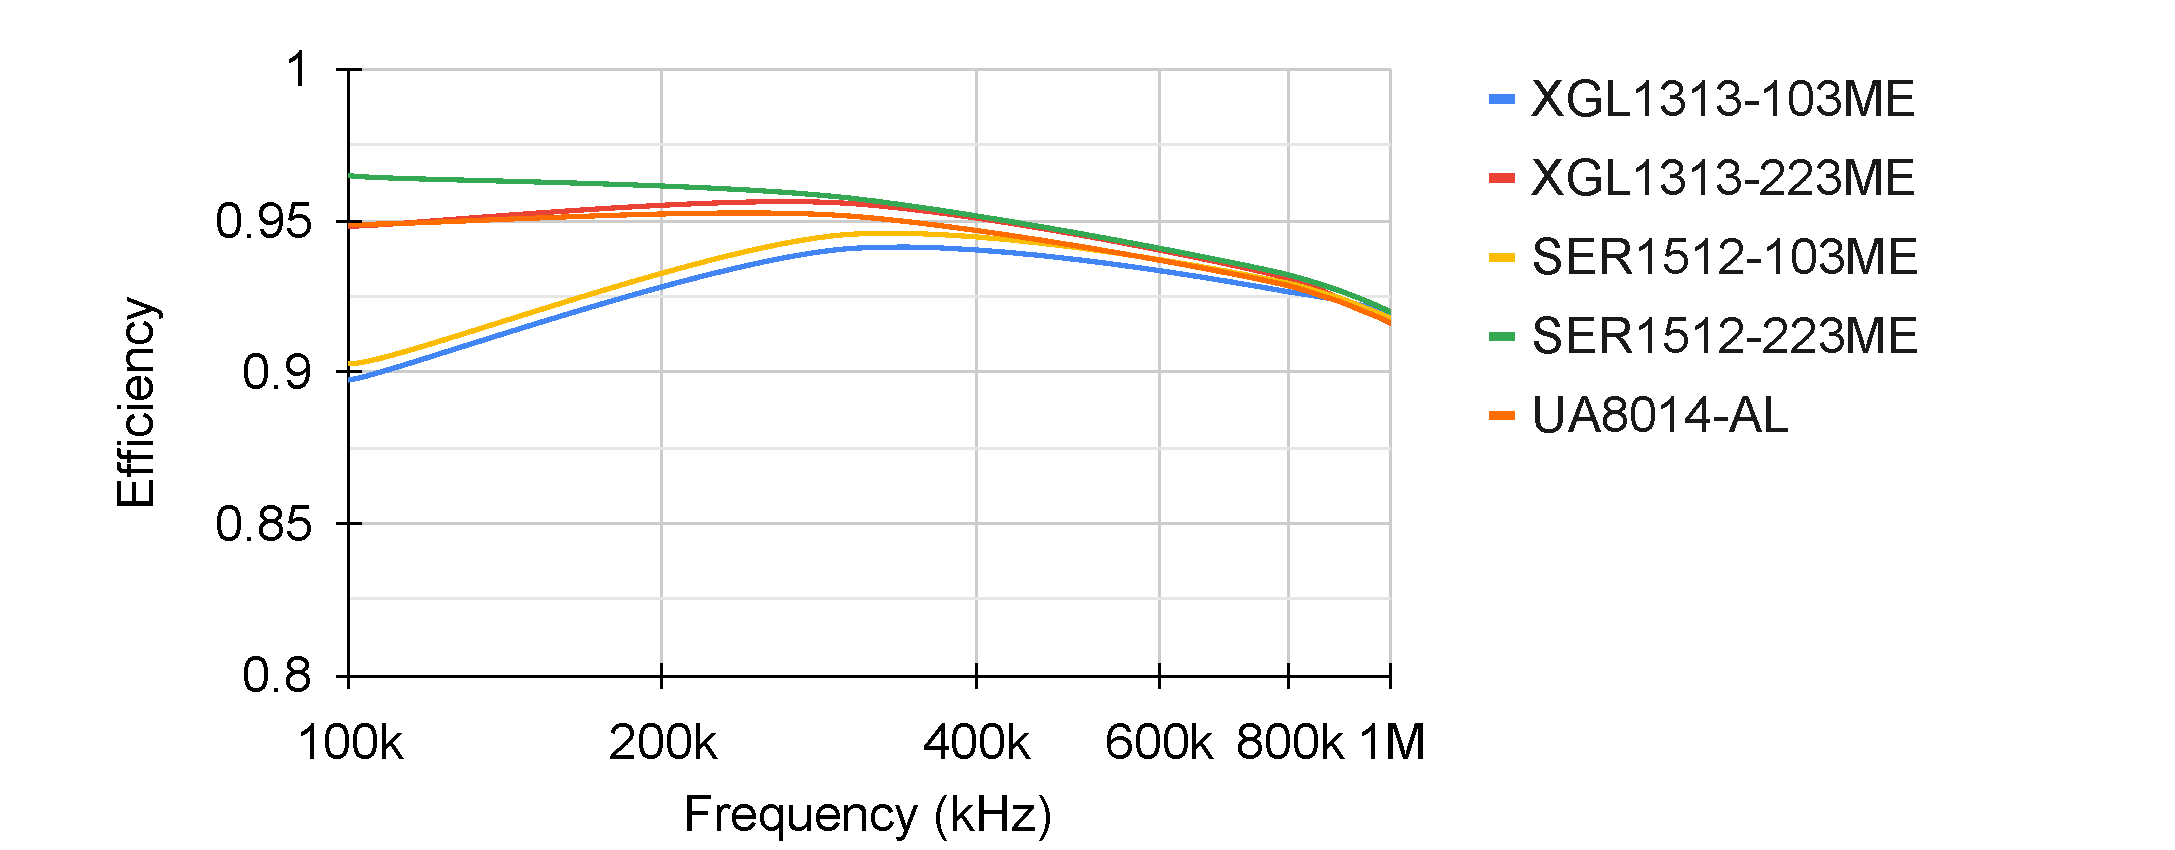
\includegraphics[width=0.95\linewidth]{Bilder//Kapitel4/BC_Meas_Efficiency_Inductor_EPC2088.pdf}
    \caption{Efficiency of the buck converter for different inductors using the \textit{EPC2088} \acp{GaNFET}}
    \label{fig:efficiency_bc_inductors}
\end{figure}
The graph can be split into two segments. For low frequencies, the inductors are the main cause of losses, dictating the behaviour of the efficiency. As inductor losses are heavily influenced by the amplitude of the ripple current, inductors with a higher inductance are more efficient at these frequencies. This is demonstrated by inductors with a similar inductance behaving alike in figure \ref{fig:efficiency_bc_inductors}. For low frequencies, the energy transported from input to output is transported in big packets and stored in the inductor. If the amount of energy in a packet gets too big, the inductor reaches saturation, increasing the ripple current and the associated core and resistive losses.\\
At high frequencies, the energy packet size shrinks, reducing the ripple current. Therefore, the losses in the inductor are now dependent on the \ac{DC} resistance and the saturation, in case of high output currents. In the measurement, the output current was kept below the saturation current, causing the losses to be dominated by the switching losses of the \acp{GaNFET}.\\
Maximum efficiency is reached in the middle between these two regions, where the combined losses are minimal.\\\\
Visualising the loss behaviour of the \textit{XGL1313-103ME} inductor and the \textit{EPC2088} \acp{GaNFET} illustrates how the combined losses come to be. 
\begin{figure}[h]
        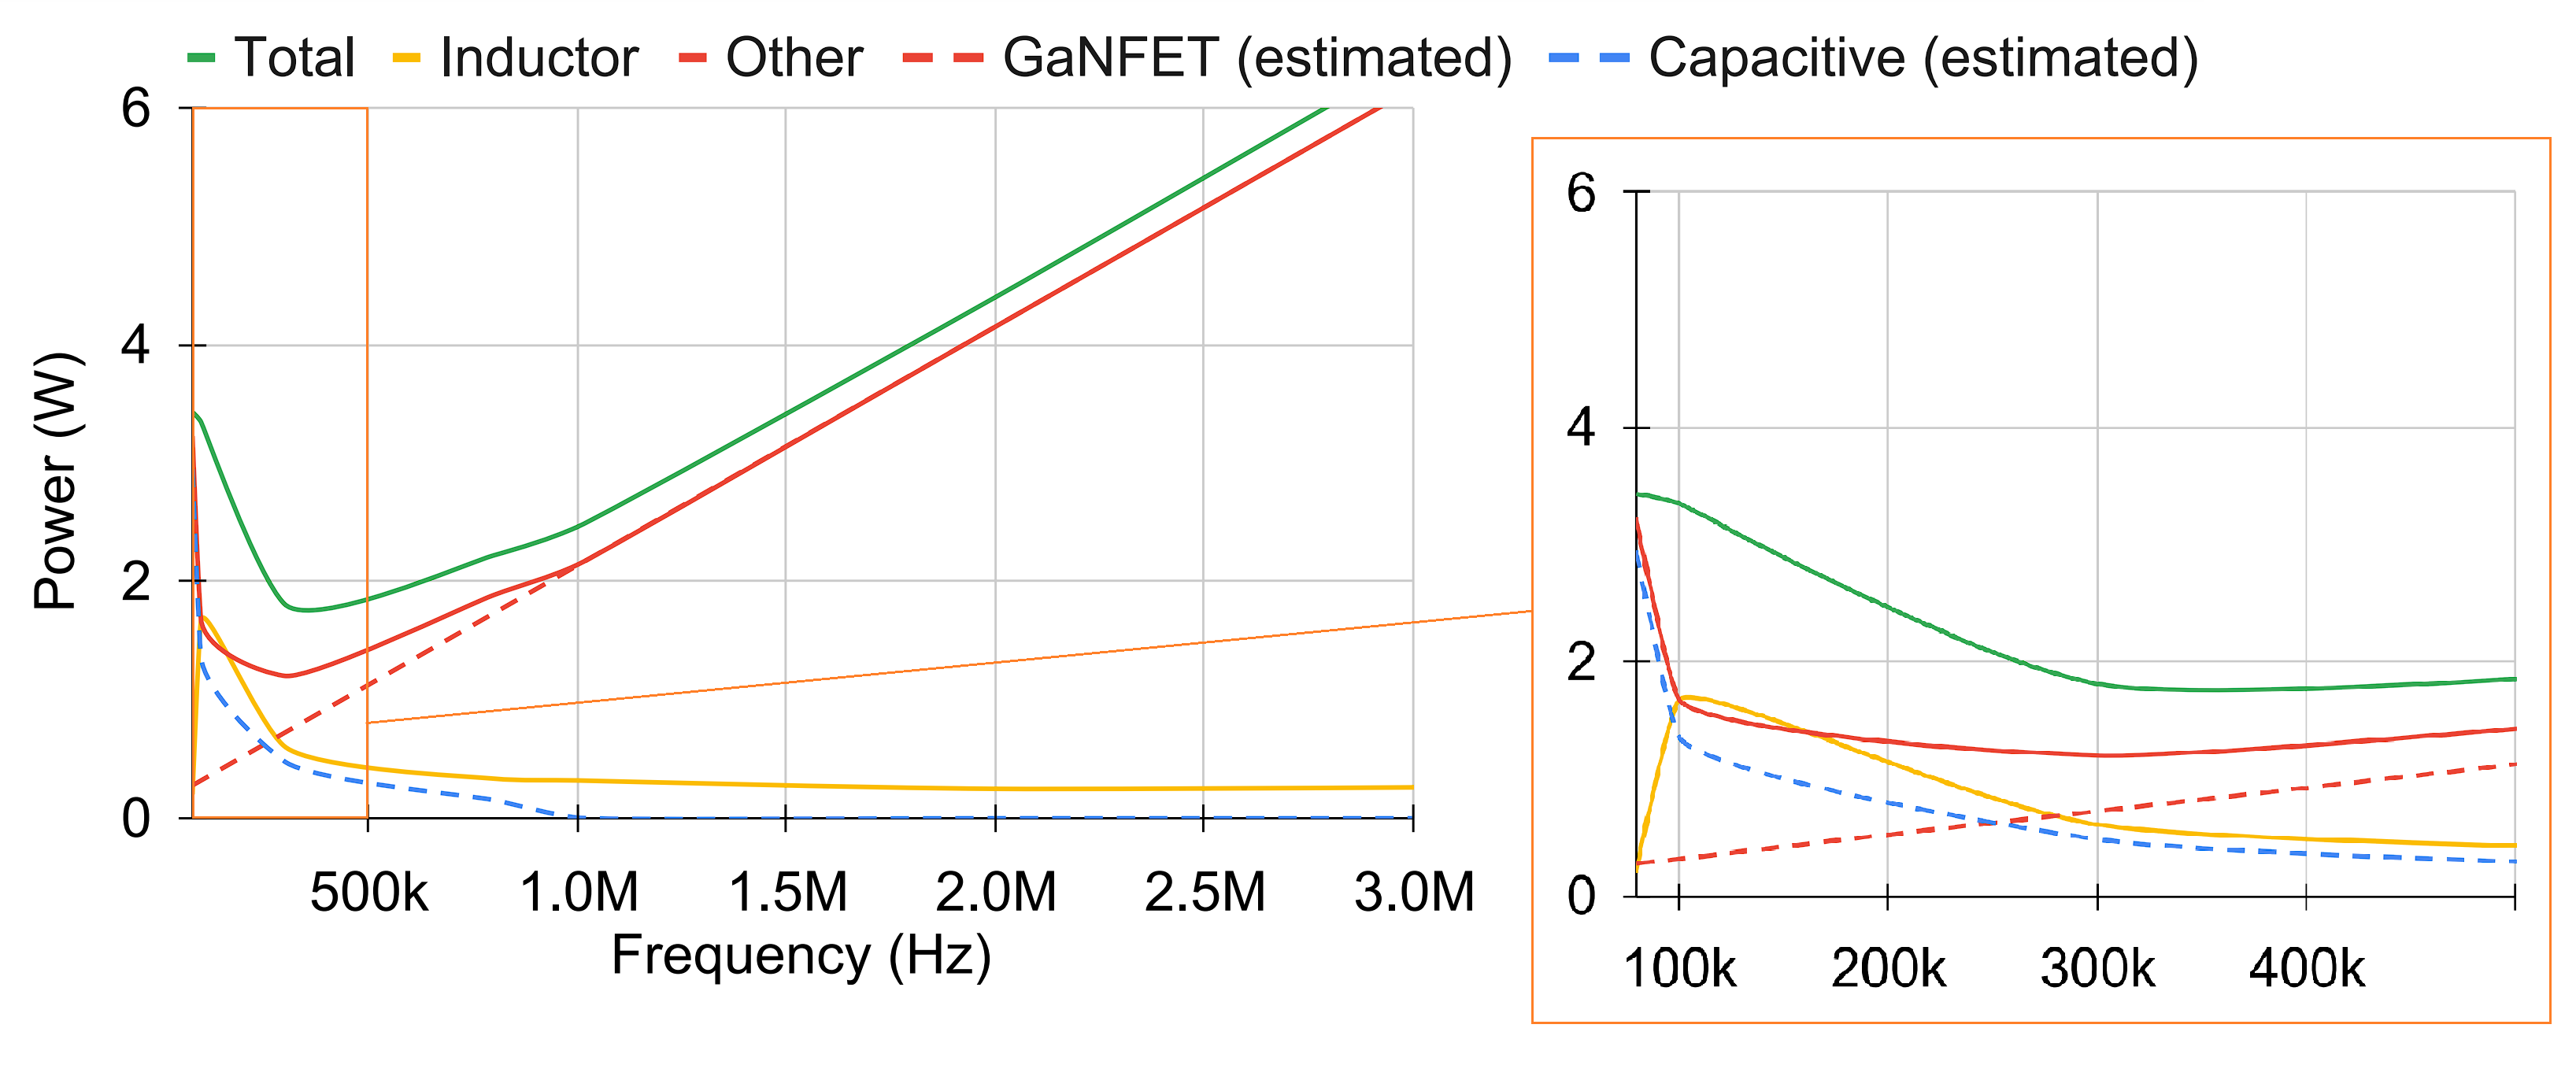
\includegraphics[width=1\textwidth]{Bilder/Kapitel4/BC_Meas_Losses_in_XGL103.png}
        \caption{Frequency dependant loss in the buck converter using the \textit{XGL1313-103ME} inductor and the \textit{EPC2088} \ac{GaNFET}}
        \label{fig:bc_losses_measured}							
\end{figure}
From the measurements, the total losses and the inductive losses can directly be extracted. The power dissipated in the \acp{GaNFET} and capacitor make up the difference between these two. Observing the behaviour of these other losses, a clear linear trend is visible for high switching frequencies, coinciding with switching losses. For these high frequencies, the capacitive losses are negligible, as the ripple current being conducted by them is minimal, as visualised by figure \ref{fig:bc_ripple_current}. Because of this, the \ac{GaNFET} losses are extrapolated linearly, as they are dictated by the dead time losses and switching losses, which are proportional to the switching frequency. The remaining losses estimate the capacitive losses. As for low frequencies the ripple current of the inductor increases, high capacitive losses are expected. The capacitor, conducting the large ripple current, dissipates large amounts of power at these frequencies, reflected by the estimated capacitive losses.
\begin{figure}[H]
    \centering
    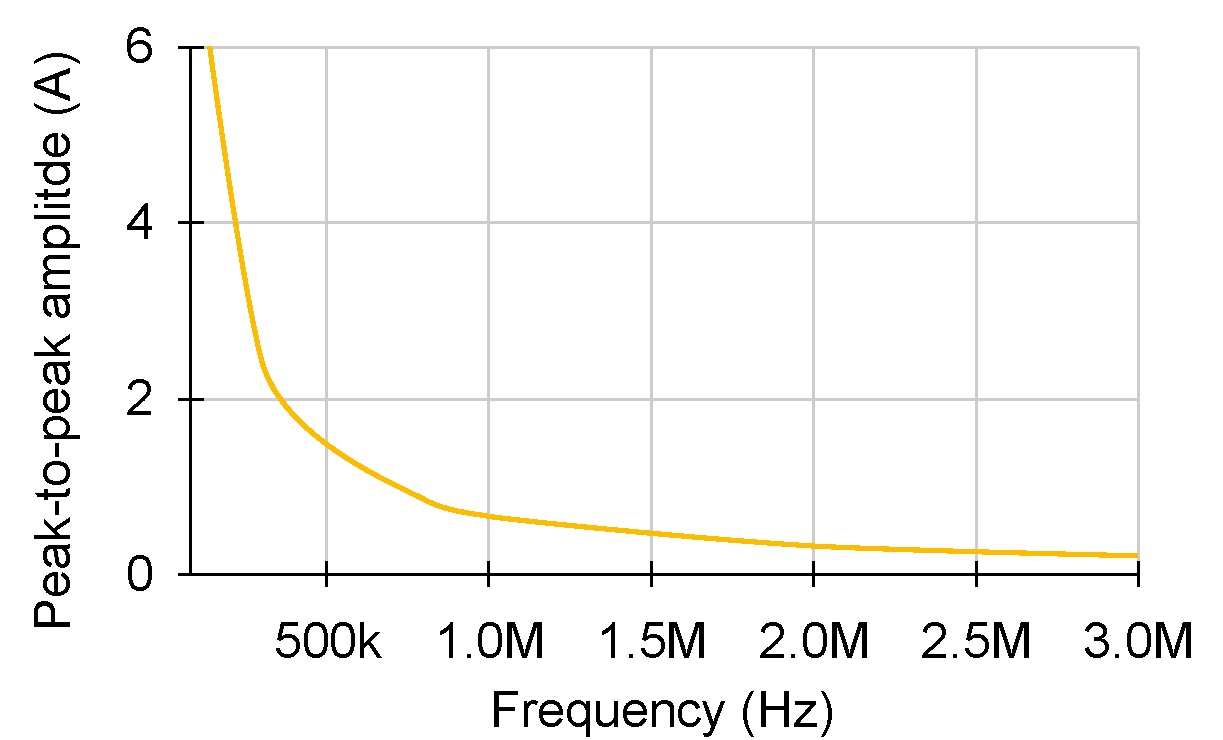
\includegraphics[width=0.6\linewidth]{Bilder//Kapitel4/BC_Meas_Ripple_Current.pdf}
    \caption{Ripple current peak to peak amplitude in the buck converter using the \textit{XGL1313-103ME} inductor and the \textit{EPC2088}}
    \label{fig:bc_ripple_current}
\end{figure}
This behaviour is mirrored by the other combinations of inductors and \acp{GaNFET} with their optimal switching frequency lying between \SI{100}{\kilo\Hz} and \SI{300}{\kilo\Hz}. 

\section{Evaluation of the Simulated Inductor}
The simulation is performed for all 20 buck converters and its results are presented here. Using the \textit{EPC2088} \ac{GaNFET} the differences in efficiency between the simulated and measured inductors are shown. As to not crowd the graph, only three of the five were chosen. The figure shows a clear correlation between the simulated and measured behaviour, with an average error in the approximation of less than 1\%. This demonstrates, that the used approach to estimate a buck converter's efficiency yields accurate results. 
\begin{figure}[H]
    \centering
    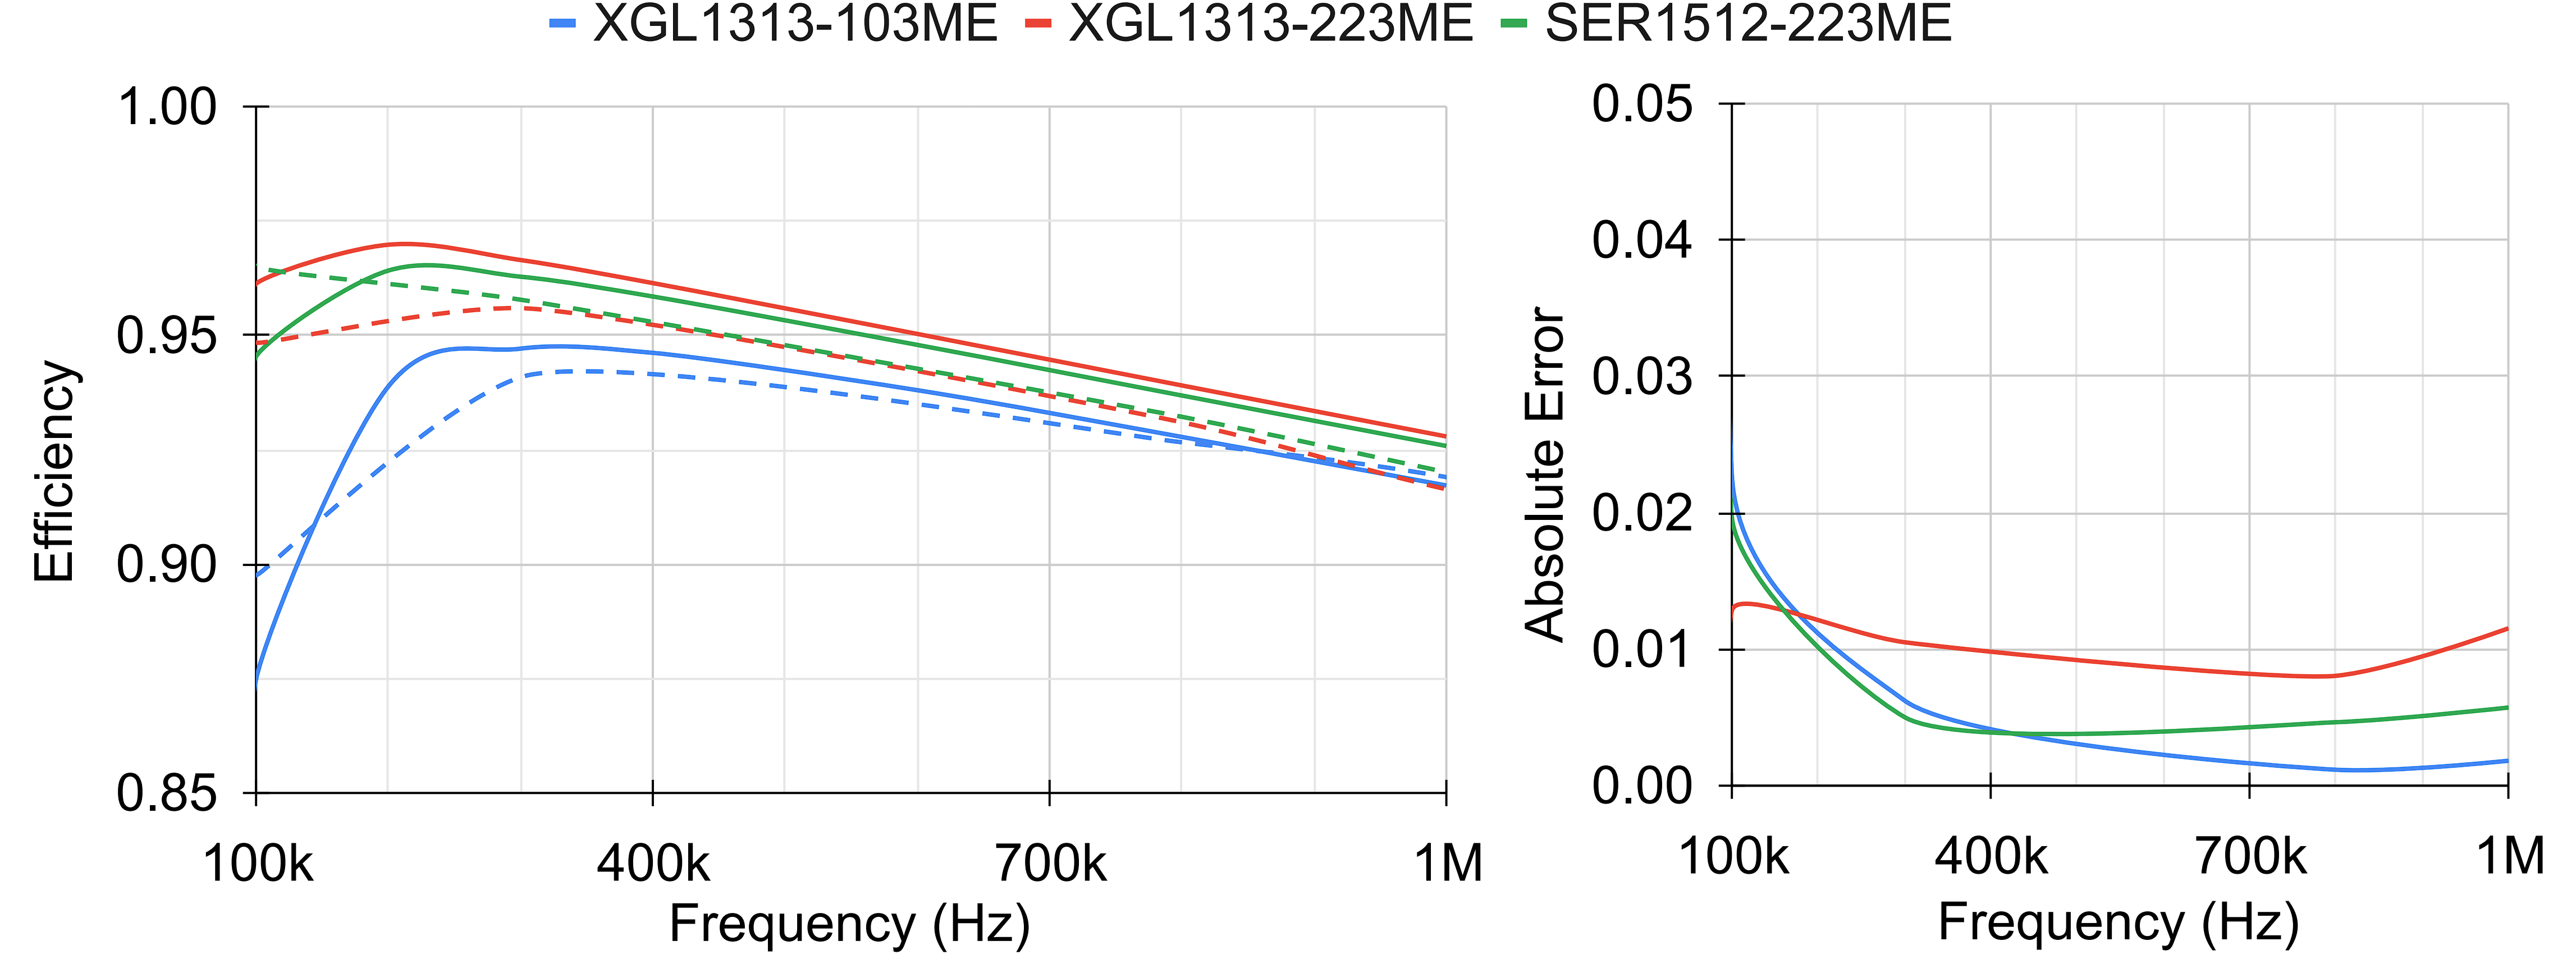
\includegraphics[width=1\linewidth]{Bilder//Kapitel4/EPC2088_Inductor_Efficiency_Comparison.png}
    \caption{Comparison of the Efficiency between the inductors}
    \label{fig:comparison_of_the_efficiency}
\end{figure}
Taking a closer look at the loss distribution of an individual buck converter, as shown in figure \ref{fig:xgl103_epc2088_loss_comparison}, gives an insight into the role of each simulated part. To keep the example used in section \ref{sec:setup_of_the_physical_buck_converter_measurement}, the buck converter using the \textit{XGL1313-103ME} inductor and the \ac{GaNFET} \textit{EPC2088} is examined. Applying the estimated switching loss and capacitive loss determined in section \ref{sec:results_of_the_bc_measurement}, the resemblance of simulated and measured losses is apparent. 
Observing the inductor, the simulated increase in the losses at low frequencies due to saturation is visible in both simulation and measurement. The \ac{GaNFET} losses increase at the same rate, differing only by a constant small wattage, due to a miss-represented conducting resistance $R_{ds_{on}}$. Losses in the capacitor also show the same behaviour, increasing rapidly as the ripple current amplitude also increases.\\ 
While the physical inductor behaviour is not completely modelled by the simulation, due to not taking into account the core losses at low frequencies and the effect of \ac{DC} bias at high frequencies, the model shows clear potential to estimate the efficiency in a buck converter. The comparison also shows the importance of incorporating the losses of the capacitor and the \ac{PCB} traces into the model. Without these the effect of inductor saturation does not result in the losses, it actually causes. In fact, even when not in saturation, the ripple current at the ideal switching frequency is not negligible and is conducted through the capacitor as well as the traces of the \ac{PCB}.\\

\begin{figure}[H]
    \centering
    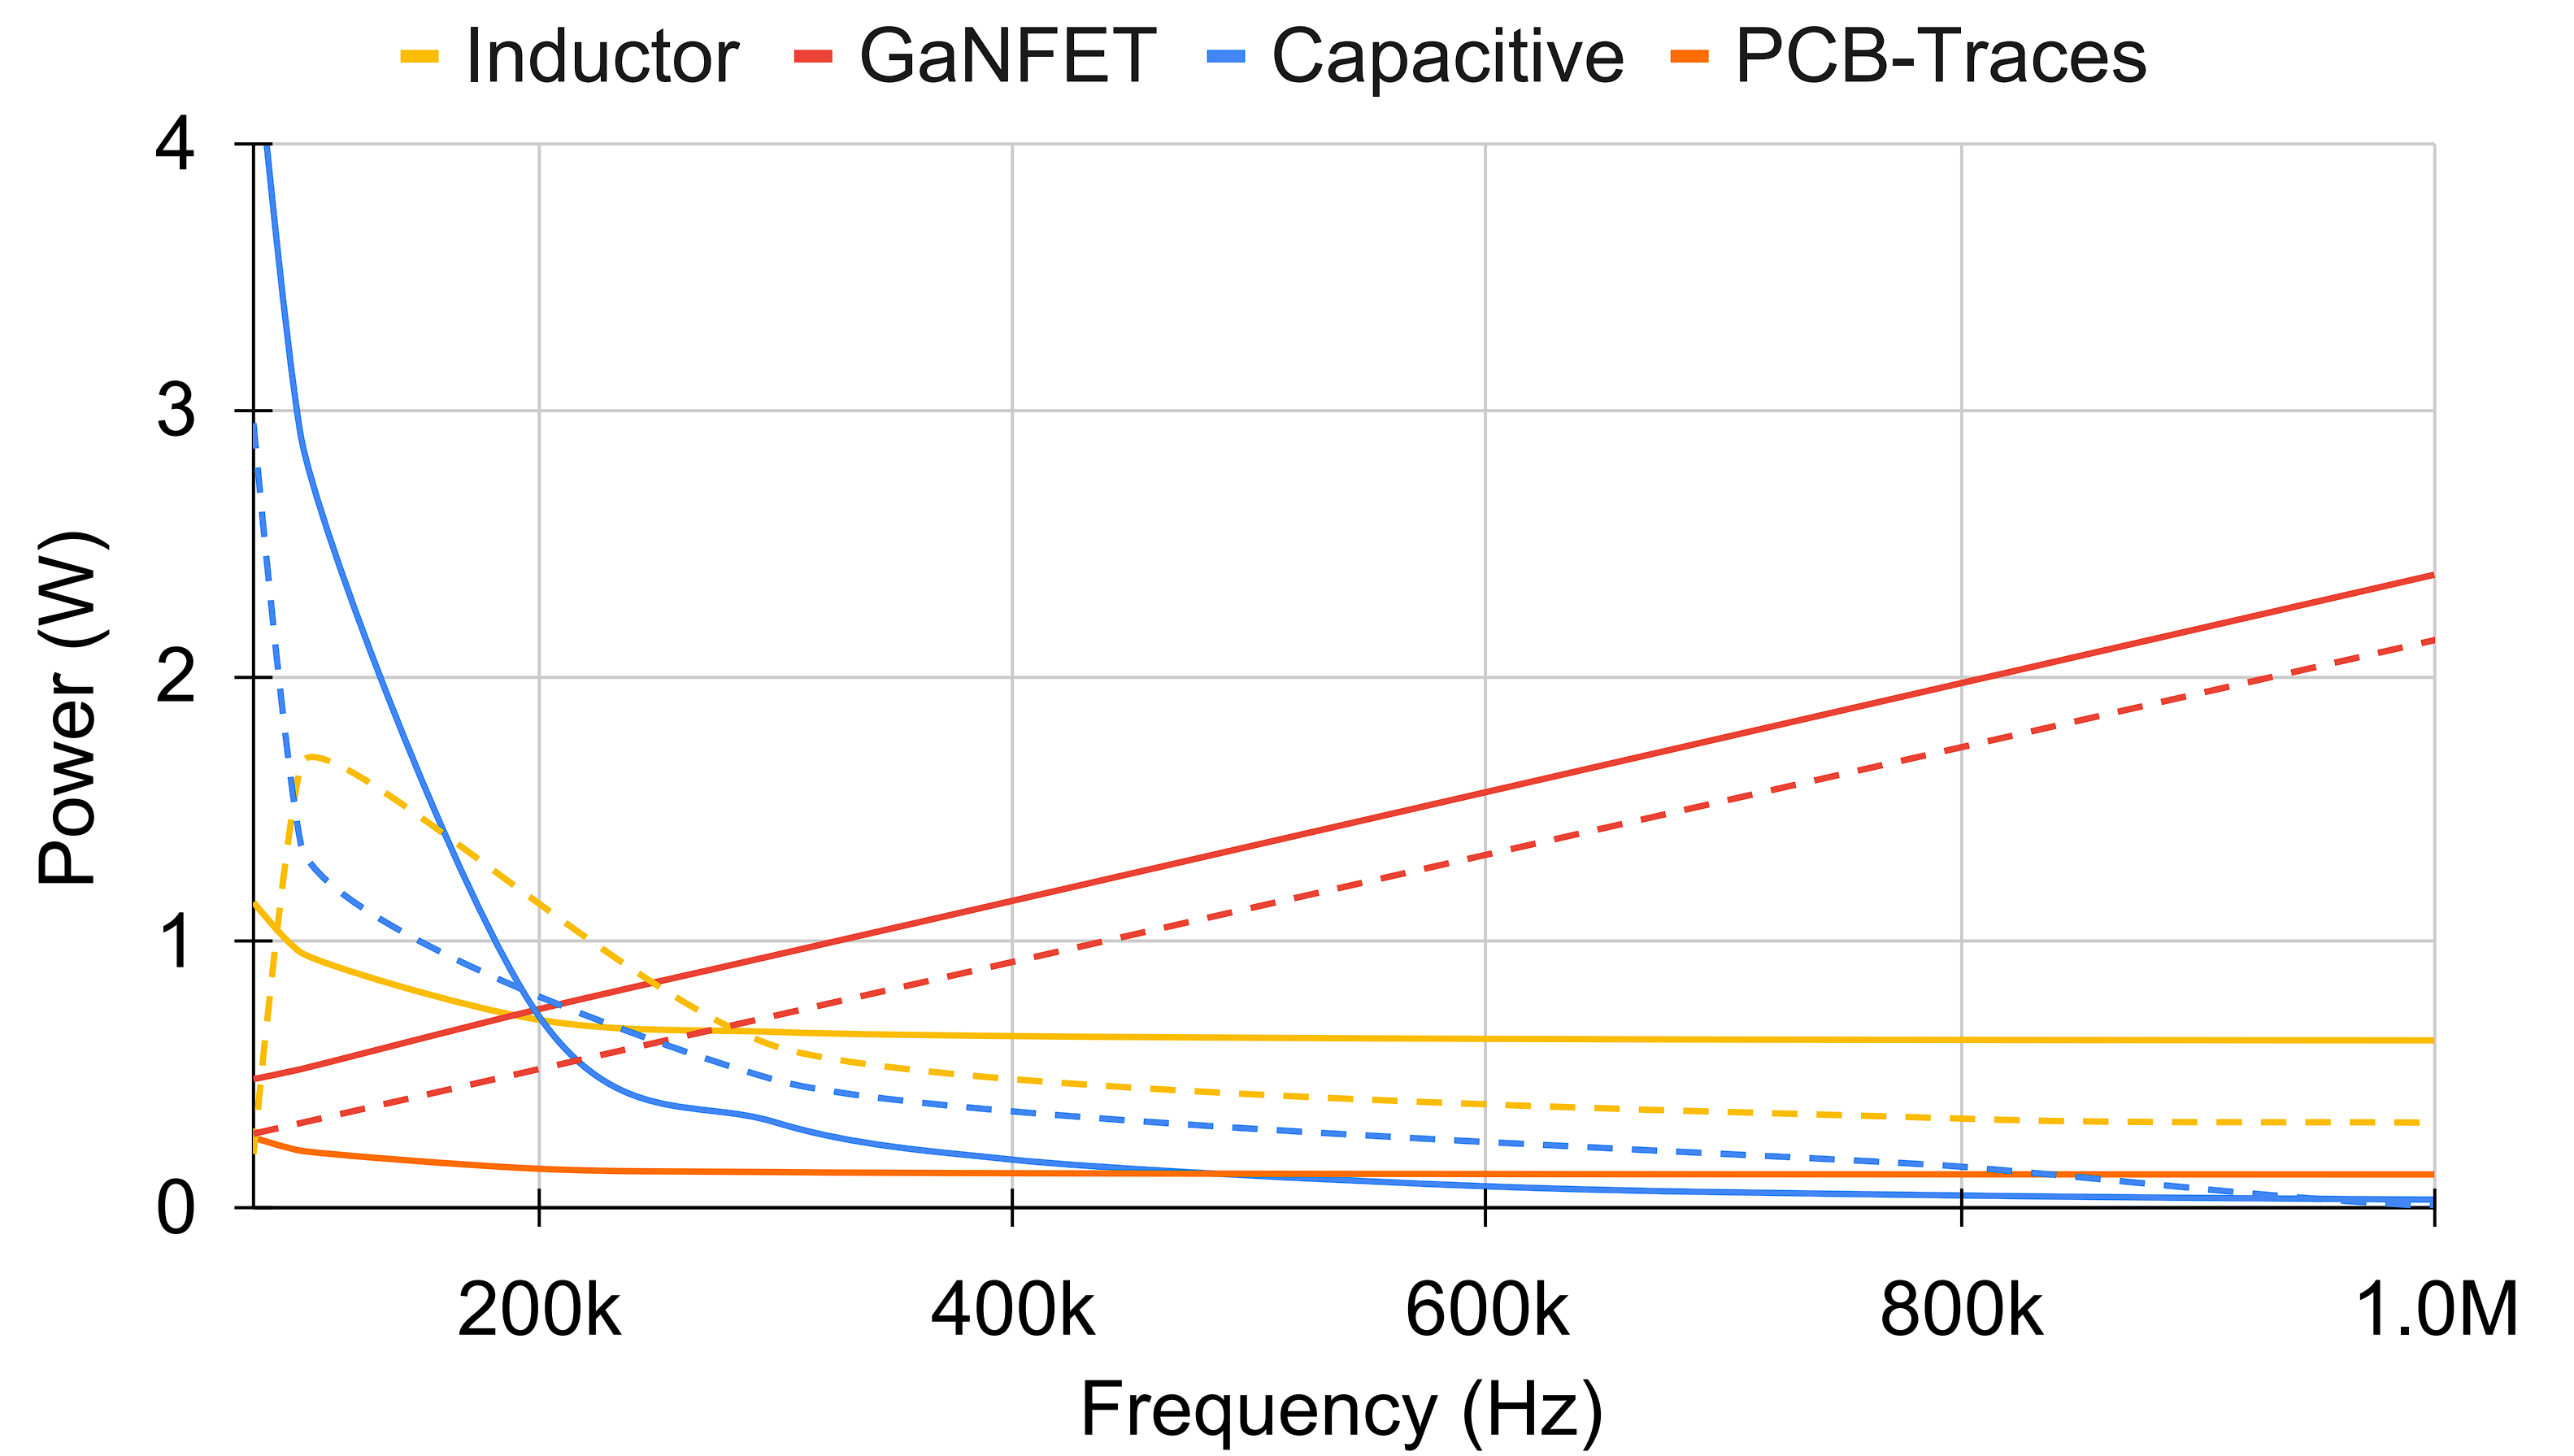
\includegraphics[width=0.85\linewidth]{Bilder/Kapitel4/XGL103_EPC2088_Simulation_Loss_Comparison.png}
    \caption{Comparison of the inductor and switching losses for the buck converter consisting of the \textit{XGL1313-103ME} inductor and \textit{EPC2088} \acp{GaNFET}}
    \label{fig:xgl103_epc2088_loss_comparison}
\end{figure}

These results show how the behaviour of a given synchronous buck converter can be approximated well by LTspice. Using industry-standard measurement equipment, the necessary parameters of any given parameters can be extracted to be used for this approach.
Incorporating the \ac{ECM} of a physical inductor with saturation into a buck converter, where the switching elements, the capacitor and the traces are represented, yields loss simulations that closely approximate the true behaviour and deliver insights about the efficiency characteristics of the observed synchronous buck converter. Using the simulation, an estimate of the ideal switching frequency and the reached efficiency at that point for a given setup can be made. It might then serve as a starting point, from which the actual ideal switching frequency is determined through measurement. While an accurate core loss model is missing in the simulation, the results still capture the behaviour to such an extent, as to clearly indicate a possible range for the ideal switching frequency.\\\\
\begin{figure}[h]
    \centering
    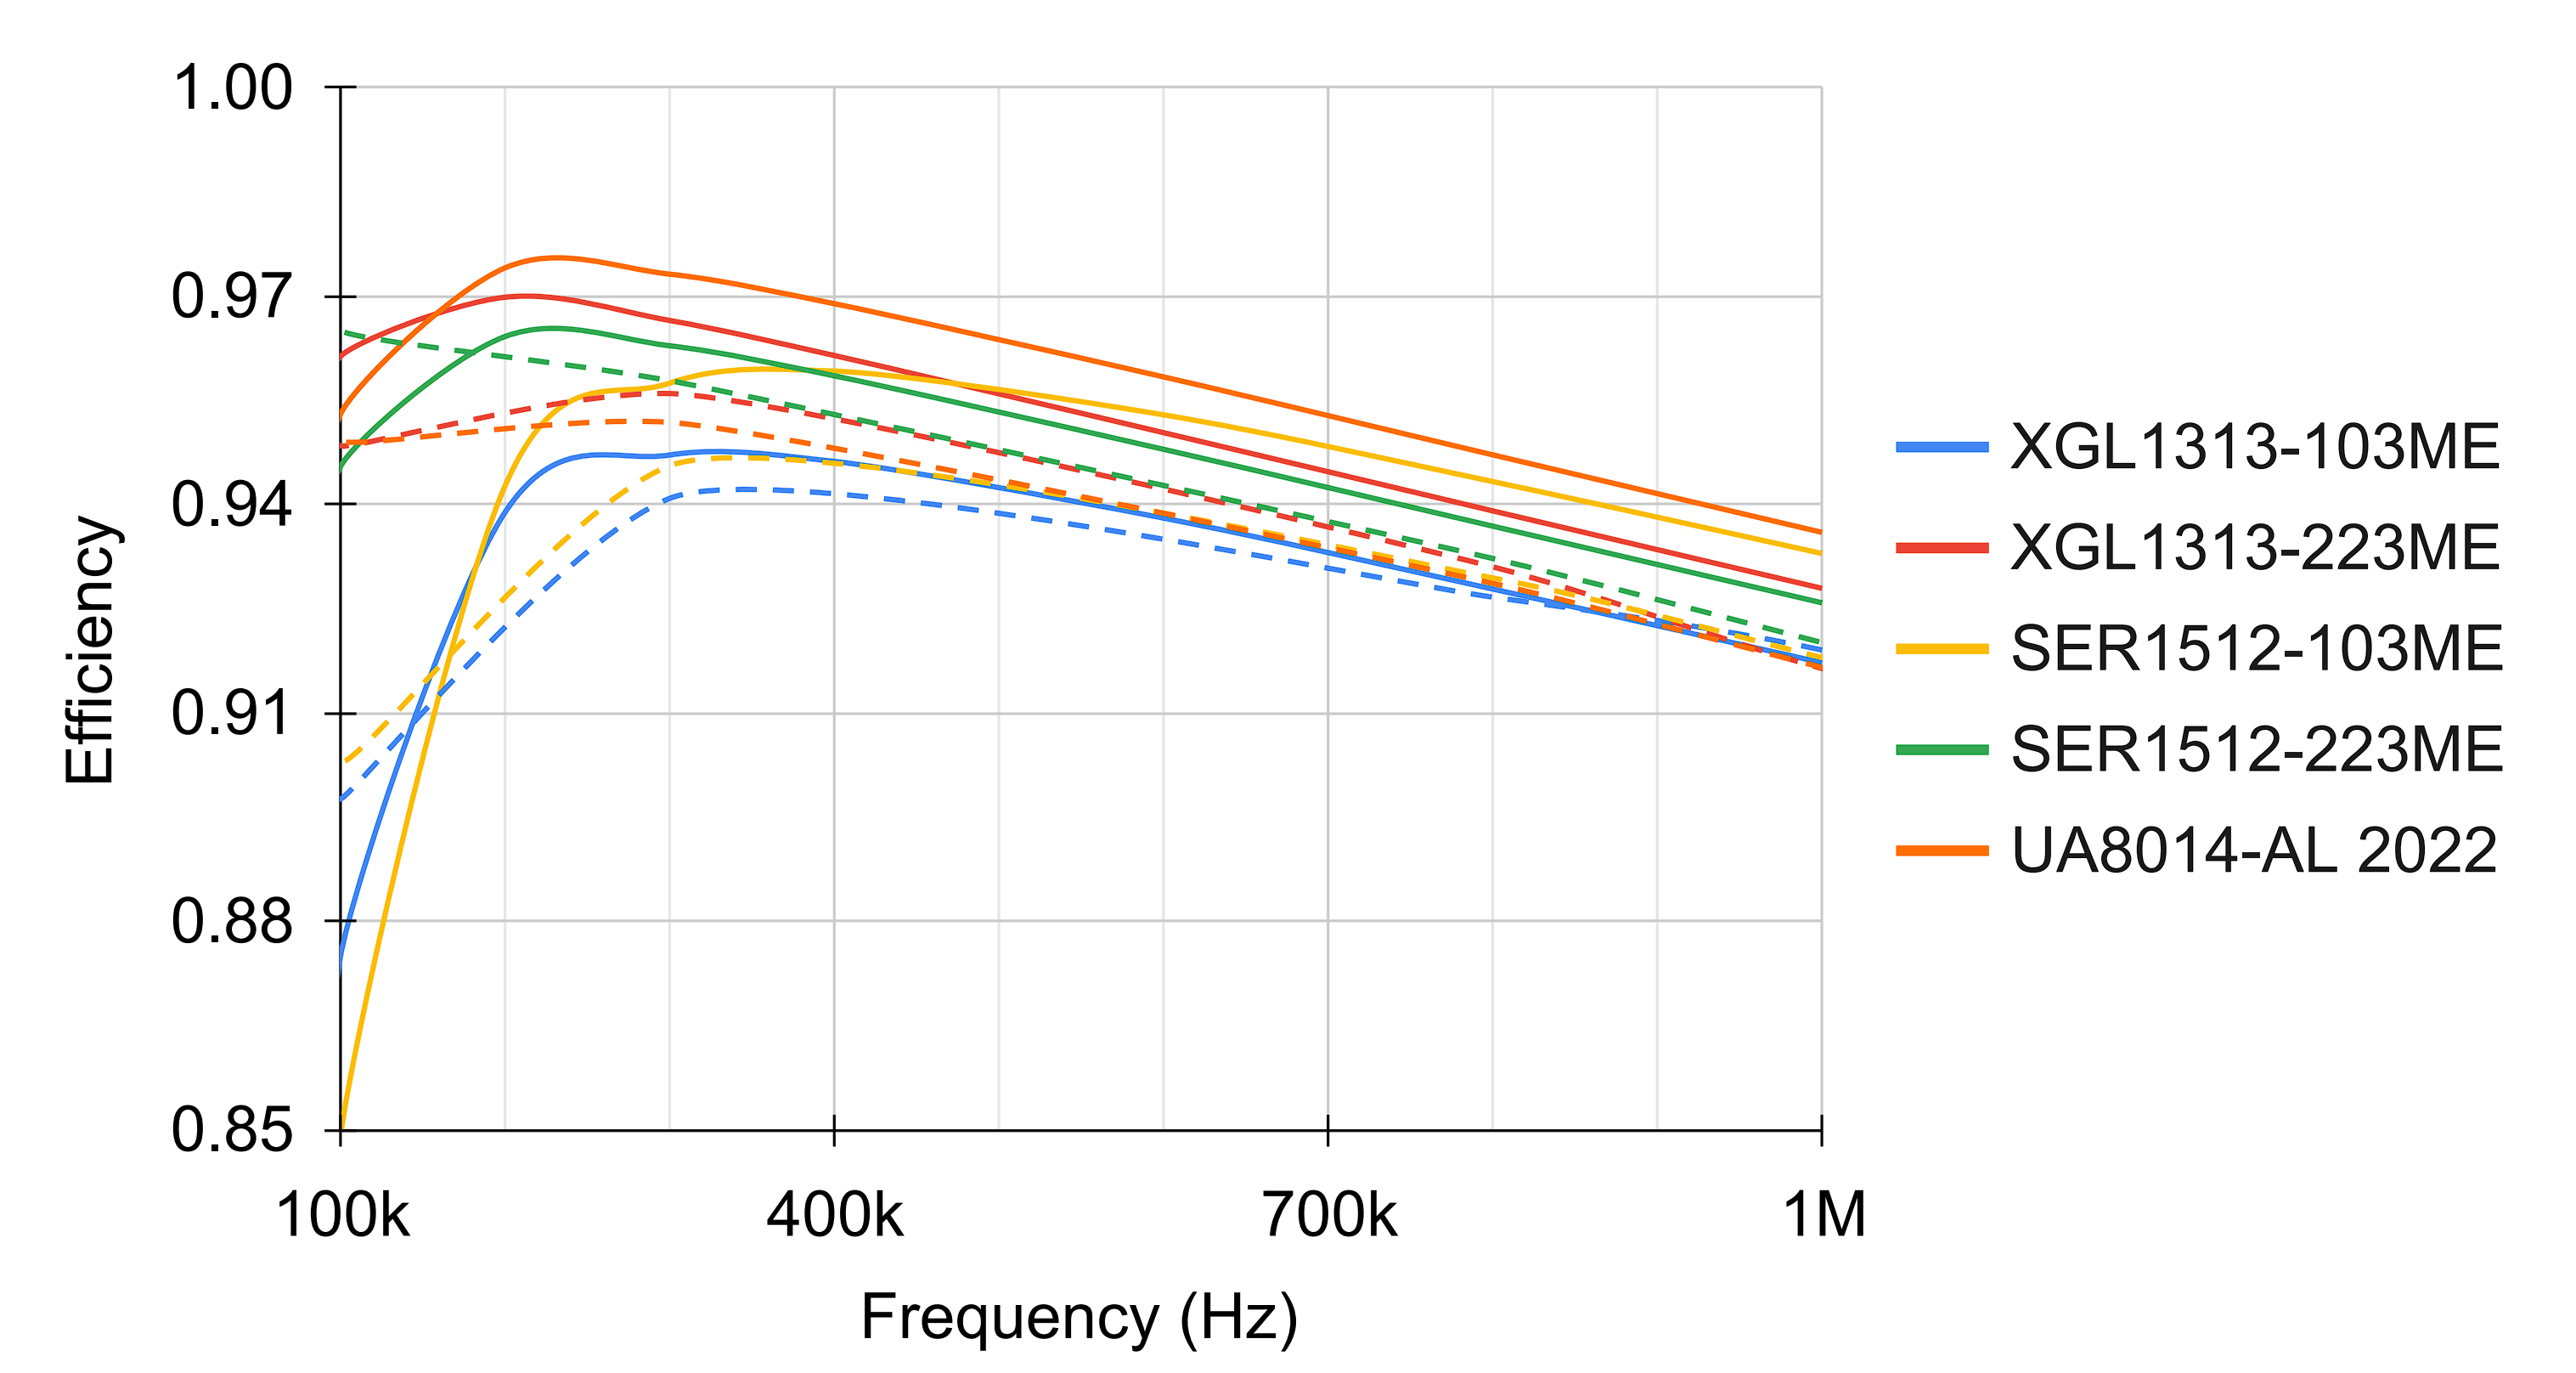
\includegraphics[width=.9\linewidth]{Bilder/Kapitel4/EPC2088_Inductor_Efficiency_Comparison_full.png}
    \caption{Comparison of the simulated and measured efficiency of the different buck converters all using the \textit{EPC2088} \ac{GaNFET} \\striped lines indicate measured values, while continuous lines are simulated}
    \label{fig:efficiency_simuilation_comparison}
\end{figure}
Furthermore, the simulations also show how the choice of the used inductor influences the maximum efficiency, that can be reached. As the point of maximum efficiency for each observed inductor lies below \SI{300}{\kilo\Hz}, the ripple current at that point has to be considered. Choosing an inductor with high inductance and a high saturation current would decrease the ripple current size, lowering the ideal switching frequency even further and increasing the maximum efficiency. Because of this, air-gaped inductors are crucial for efficient \ac{SMPS}, as they have a much larger saturation current.\\
Concerning the output capacitance of the buck converter, the results of figure \ref{fig:xgl103_epc2088_loss_comparison} show it to be the main contributor to power loss in the low-frequency range. Because of this, the chosen electrolytic capacitor is not suited for reaching high efficiency in this setup. Through the simulation, this is able to be verified, without directly measuring the power dissipation in the capacitor. Exchanging the capacitor for a ceramic capacitor with a lower \ac{ESR} would increase the maximum efficiency and lower the optimal switching frequency.